\subsection{Practical use}

\begin{frame}{$\mathcal{O}$-Notation}{Practical use}
  \textbf{Practical use:}
  \begin{itemize}
    \item
      It is much easier to determine the runtime of an algorithm by using
      the $\mathcal{O}$-Notation
    \begin{enumerate}
      \item
        Computing rules
      \item
        Practical use
    \end{enumerate}
  \end{itemize}
\end{frame}

%-------------------------------------------------------------------------------

\begin{frame}{$\mathcal{O}$-Notation}{Characteristics}
  \begin{itemize}
    \item
      Transitivity:
      \begin{eqnarray*}
        f \in \Theta(g) \; \wedge \; g \in \Theta(h)
       \onslide<2- |handout:1>{& \rightarrow & f \in \Theta(h)}\\
       f \in \mathcal{O}(g) \; \wedge \; g \in \mathcal{O}(h)
       \onslide<3- |handout:1>{ & \rightarrow & f \in \mathcal{O}(h)}\\
       f \in \Omega(g) \; \wedge  \; g \in \Omega(h)
       \onslide<4- |handout:1>{& \rightarrow & f \in \Omega(h)}
      \end{eqnarray*}
    \item<5- |handout:1>
      Symmetry:
      \begin{eqnarray*}
        f \in \Theta(g) & \leftrightarrow & g \in \Theta(f)\\
        \onslide<6- |handout:1>{f \in \mathcal{O}(g)}
        \onslide<7- |handout:1>{& \leftrightarrow & g \in \Omega(f)}
      \end{eqnarray*}
    \item<8- |handout:1>
      Reflexivity:
      \begin{eqnarray*}
        f \in \Theta(f) & f \in \Omega(f) & f \in \mathcal{O}(f)
      \end{eqnarray*}
  \end{itemize}
\end{frame}

%-------------------------------------------------------------------------------

\begin{frame}{$\mathcal{O}$-Notation}{Calculation Rules}
  \begin{itemize}
    \item
      Trivial:
      \begin{eqnarray*}
        f & \in & \mathcal{O} (f)\\
        k \cdot \mathcal{O} (f) & = & \mathcal{O} (f)\\
        \mathcal{O} (f + k) & = & \mathcal{O} (f)
      \end{eqnarray*}
    \item
      Addition:
      \begin{eqnarray*}
        \mathcal{O} (f) + \mathcal{O} (g) & = & \mathcal{O} 
        (\mathrm{max}\{f,\;g\})
      \end{eqnarray*}
    \item
      Multiplication:
      \begin{eqnarray*}
        \mathcal{O} (f) \cdot \mathcal{O} (g) & = & \mathcal{O} (f \cdot g)
      \end{eqnarray*}
  \end{itemize}
\end{frame}

%-------------------------------------------------------------------------------

\begin{frame}{$\mathcal{O}$-Notation}{Runtime Complexity}
  \begin{itemize}
    \item
      The input size for all examples is $n$
    \item
      Basic operations
  \end{itemize}
  \begin{tabularx}{\linewidth}{P{11em}O{4em}}
    i1 = 0 & $\mathcal{O}(1)$
  \end{tabularx}
  \begin{itemize}
    \item
      Sequences of basic operations
  \end{itemize}
  \begin{tabularx}{\linewidth}{P{11em}O{4em}O{1.75em}L}
    i1 = 0 & $\mathcal{O}(1)$ & {} & {}\\
    i2 = 0 & $\mathcal{O}(1)$ & {} & {}\\
    $\cdots$ & $\cdots$ & {} & {}\\
    i327 = 0 & $\mathcal{O}(1)$ &
    \hspace*{-0.5em}%
    \multirow{-4}{*}{$\left.%
        \begin{array}{@{}c@{}}\\[3em]\end{array}%
      \right\rbrace$} &%
    \multirow{-4}{*}{$327 \cdot \mathcal{O}(1) = \mathcal{O}(1)$}%
  \end{tabularx}
\end{frame}

%-------------------------------------------------------------------------------

\begin{frame}{$\mathcal{O}$-Notation}{Runtime Complexity}
  \begin{itemize}
    \item
      Loops
  \end{itemize}
  \begin{tabularx}{\linewidth}{P{11em}O{4em}O{1.75em}L}
    for i in range(0, n): & $\mathcal{O}(n)$ & {} & {}\\%
    \hhline{~*{1}{-}}%
    $\hspace*{1.5em}$ a[i] = 0 & $\mathcal{O}(1)$ &%
    \multirow{-2}{*}{%
      $\left.\begin{array}{@{}c@{}}\\[1em]\end{array}\right\rbrace$}&%
    \multirow{-2}{*}{$\mathcal{O}(1) \cdot \mathcal{O}(n) = \mathcal{O}(n)$}%
  \end{tabularx}\\[0.5em]
  \begin{tabularx}{\linewidth}{P{11em}O{4em}O{1.75em}O{5em}O{1.75em}L}
    for i in range(0, n): & $\mathcal{O}(n)$ & {} & {} & {} & {}\\
    \hhline{~*{3}{-}}
    $\hspace*{1.5em}$ a1[i] = 0 & $\mathcal{O}(1)$ & {} & {} & {} & {}\\
    $\hspace*{1.5em} \cdots$ & $\cdots$ & {} & {} & {} & {}\\
    $\hspace*{1.5em}$ a137[i] = 0 & $\mathcal{O}(1)$ &
    \multirow{-3}{*}{$\left.
        \begin{array}{@{}c@{}}\\[2em]\end{array}
      \right\rbrace$} &
    \multirow{-3}{*}{
      $\begin{array}{@{}c@{}}
        137 \cdot \mathcal{O}(1)\\
        = \mathcal{O}(1)
      \end{array}$
    } &
    \multirow{-4}{*}{$\left.
        \begin{array}{@{}c@{}}\\[3em]\end{array}
      \right\rbrace$} &
    \multirow{-4}{*}{
      $\begin{array}{@{}c@{}}
      \mathcal{O}(1) \cdot \mathcal{O}(n)\\
      = \mathcal{O}(n)
      \end{array}$
    }
  \end{tabularx}
\end{frame}

%-------------------------------------------------------------------------------

\begin{frame}{$\mathcal{O}$-Notation}{Runtime Complexity}
  \begin{itemize}
    \item
      Loops
   \end{itemize}
  \begin{tabularx}{\textwidth}{P{11em}O{4.75em}O{1.75em}O{4.5em}O{1.75em}L}
    for i in range(0, n): & $\mathcal{O}(n)$ & {} & {} & {} & {}\\
    \hhline{~*{1}{-}}
    $\hspace*{1.5em}$ for j in range(0, n-1): & $\mathcal{O}(n-1)$ &
    \multirow{-2}{*}{$\left.%
        \begin{array}{@{}c@{}}\\[1em]\end{array}%
      \right\rbrace$} &%
    \multirow{-2}{*}{%
      $\begin{array}{@{}c@{}}%
        \mathcal{O}(n) \cdot \mathcal{O}(n)\\%
        = \mathcal{O}(n^2)%
      \end{array}$%
    } & {} & {}\\
    \hhline{~*{3}{-}}
    $\hspace*{3em}$ a1[i][j] = 0 & $\mathcal{O}(1)$ & {} & {} & {} & {}\\
    $\hspace*{3em} \cdots$ & $\cdots$ & {} & {} & {} & {}\\
    $\hspace*{3em}$ a137[i][j] = 0 & $\mathcal{O}(1)$ &
    \multirow{-3}{*}{$\left.
      \begin{array}{@{}c@{}}\\[2em]\end{array}
      \right\rbrace$} &
    \multirow{-3}{*}{
      $\begin{array}{@{}c@{}}
      137 \cdot \mathcal{O}(1)\\
      = \mathcal{O}(1)
      \end{array}$
    } &%
    \multirow{-5}{*}{$\left.
      \begin{array}{@{}c@{}}\\[4.5em]\end{array}
      \right\rbrace$} &%
    \hspace*{-0.5em}%
    \multirow{-5}{*}{%
      $\begin{array}{@{}c@{}}
      \mathcal{O}(1) \cdot \mathcal{O}(n^2)\\
      = \mathcal{O}(n^2)
      \end{array}$
    }%
  \end{tabularx}
\end{frame}

%-------------------------------------------------------------------------------

\begin{frame}{$\mathcal{O}$-Notation}{Runtime Complexity}
  \begin{itemize}
    \item
      Conditions
  \end{itemize}
  \begin{tabularx}{\textwidth}{P{11em}O{4em}O{1.75em}O{4.5em}O{1.75em}L}
    if x < 100: & $\mathcal{O}(1)$ & {} & {} & {} & {}\\
    \hhline{~*{1}{-}}
    $\hspace*{1.5em}$ y = x & $\mathcal{O}(1)$ &
    \multirow{-2}{*}{$\left.%
      \begin{array}{@{}c@{}}\\[1em]\end{array}%
      \right\rbrace$} &%
    \multirow{-2}{*}{$\mathcal{O}(1)$} & {} & {}\\
    else: & {} & {} & {} & {} & {}\\
    $\hspace*{1.5em}$ for i in range(0, n): & $\mathcal{O}(n)$ &
    {} & {} & {} & {}\\
    \hhline{~*{1}{-}}
    $\hspace*{3em}$ if a[i] > y: & $\mathcal{O}(1)$ & {} & {} & {} & {}\\
    \hhline{~*{1}{-}}
    $\hspace*{4.5em}$ y = a[i] & $\mathcal{O}(1)$ &
    \multirow{-3}{*}{$\left.
      \begin{array}{@{}c@{}}\\[2em]\end{array}
      \right\rbrace$} &
    \multirow{-3}{*}{
      $\begin{array}{@{}c@{}}
      \mathcal{O}(n) \cdot \mathcal{O}(1)\\
      = \mathcal{O}(n)
      \end{array}$
    } &%
    \multirow{-6}{*}{$\left.
      \begin{array}{@{}c@{}}\\[5.5em]\end{array}
      \right\rbrace$} &%
    \hspace*{-0.5em}%
    \multirow{-6}{*}{%
      $\begin{array}{@{}c@{}}
      \mathcal{O}(\max\{1,n\})\\
      = \mathcal{O}(n)
      \end{array}$
    }%
  \end{tabularx}
\end{frame}

%-------------------------------------------------------------------------------

\codeslide{python}{
\begin{frame}{$\mathcal{O}$-Notation}{Arithmetic mean}
  \begin{itemize}
    \item
      {\color{MainA}Input:} List $x$ with $n$ numbers
    \item
      {\color{MainA}Output:} $a[i]$ is the arithmetic mean of $x[0]$
      to $x[i]$
  \end{itemize}
  \lstinputlisting[
    language=Python,
    style={python-idle-code},
    basicstyle=\small,
    tabsize=4,
    emph={arithMean},
    emphstyle=\color{blue}
  ]{Code/ArithmeticMean/ArithmeticMean.py}
\end{frame}
}

%-------------------------------------------------------------------------------

\codeslide{java}{
\begin{frame}{$\mathcal{O}$-Notation}{Arithmetic mean}
  \begin{itemize}
    \item
      {\color{MainA}Input:} Array $x$ with $n$ numbers
    \item
      {\color{MainA}Output:} $a[i]$ is the arithmetic mean of $x[0]$
      to $x[i]$
  \end{itemize}
  \lstinputlisting[
    language=Java,
    style={java-eclipse-code},
    basicstyle=\small,
    tabsize=4,
    emph={arithMean},
    emphstyle=\color{blue}
  ]{Code/ArithmeticMean/ArithmeticMean.java}
\end{frame}
}

%-------------------------------------------------------------------------------

\codeslide{cpp}{
\begin{frame}{$\mathcal{O}$-Notation}{Arithmetic mean}
  \begin{itemize}
    \item
      {\color{MainA}Input:} Vector $x$ with $n$ numbers
    \item
      {\color{MainA}Output:} $a[i]$ is the arithmetic mean of $x[0]$
      to $x[i]$
  \end{itemize}
  \lstinputlisting[
    language=C++,
    style={cpp-eclipse-code},
    basicstyle=\small,
    tabsize=4,
    emph={arith_mean},
    emphstyle=\color{blue}
  ]{Code/ArithmeticMean/ArithmeticMean.cpp}
\end{frame}
}

%-------------------------------------------------------------------------------

\begin{frame}{$\mathcal{O}$-Notation Runtime complexity}
 \begin{tabularx}{\textwidth}{P{11em}O{4.75em}O{1.75em}O{3em}O{1.75em}L}
   for i in range(0, len(x)): & $\mathcal{O}(n)$ & {} & {} & {} & {}\\
   \hhline{~*{1}{-}}
   $\hspace*{1.5em}$ s = 0 & $\mathcal{O}(1)$ &
   \multirow{-2}{*}{$\left.%
     \begin{array}{@{}c@{}}\\[1em]\end{array}%
     \right\rbrace$} &%
    \multirow{-2}{*}{$\mathcal{O}(n)$} & {} & {}\\
    \hhline{~*{3}{-}}
    $\hspace*{1.5em}$ for j in range(0, i+1): & $\mathcal{O}(i+1)$ &
    {} & {} & {} & {}\\
    \hhline{~*{1}{-}}
    $\hspace*{3em}$ s = s + x[j] & $\mathcal{O}(1)$ &
    \multirow{-2}{*}{$\left.%
      \begin{array}{@{}c@{}}\\[1em]\end{array}%
      \right\rbrace$} &%
    \multirow{-2}{*}{$\mathcal{O}(i)$} & {} & {}\\
    \hhline{~*{3}{-}}
    $\hspace*{1.5em}$ a[i] = s / (i+1) & $\mathcal{O}(1)$ & {} & {} &
    \multirow{-5}{*}{$\left.
      \begin{array}{@{}c@{}}\\[4.5em]\end{array}
      \right\rbrace$} &%
    \hspace*{-0.5em}%
    \multirow{-5}{*}{%
      $\begin{array}{@{}c@{}}
      \mathcal{O}(n) \cdot \mathcal{O}(i)\\
      = \mathcal{O}(n^2)
      \end{array}$
    }%
  \end{tabularx}
  \begin{itemize}
    \item
      How often will the instructions in the loop be executed,
      when the problem has size $n$?
  \end{itemize}
  \[1 + 2 + \ldots + n = \dfrac{n \cdot (n + 1)}{2} \in \mathcal{O} (n^2)\]
\end{frame}

%-------------------------------------------------------------------------------

\begin{frame}{$\mathcal{O}$-Notation}{Discussion}
  \textbf{Way of speaking:}
  \begin{itemize}
    \item
      With the $\mathcal{O}$-Notation we look at the behavior of a function when
      $n \to \infty$
    \item
      We only analyze the runtime when $n \geq n_0$
    \item
      We talk about {\color{MainA}asymptotic analysis}, when we discuss 
      cost, runtime, etc. as $\mathcal{O}(\ldots)$, $\Omega(\ldots)$
      or $\Theta(\ldots)$
  \end{itemize}
\end{frame}

%-------------------------------------------------------------------------------

\begin{frame}{$\mathcal{O}$-Notation}{Discussion}
  \begin{alertblock}{\textbf{Attention:}}
    \begin{itemize}
      \item
        If you are using \textbf{asymptotic analysis}, you can not make any
        predictions about the runtime of smaller input sizes ($n < n_0$)
      \item
        For small input sizes (mostly $n < 10$),
        the runtime is predictably small
      \item
        $n_0$ does not necessarily have to be small
    \end{itemize}
  \end{alertblock}
\end{frame}

%-------------------------------------------------------------------------------

\begin{frame}{$\mathcal{O}$-Notation}{Discussion}
  \textbf{Examples:}
  \begin{itemize}
    \item
    Let A and B be algorithms
    \begin{itemize}
      \item
        A has the runtime $f(n) = 80 \, n$
      \item
        B has the runtime $f(n) = 2 \, n \, \log_2 n$
    \end{itemize}
    \item
      So $f = \mathcal{O}(g)$ but \textbf{not} $\Theta(g)$
      \begin{itemize}
        \item
          $\Rightarrow$ A is asymptotic faster than B
        \item
          $\Rightarrow$
          There is a $n_0$ for that $n \geq n_0\!: \; f(n) \leq g(n)$
      \end{itemize}
  \end{itemize}
\end{frame}

%-------------------------------------------------------------------------------

\begin{frame}{$\mathcal{O}$-Notation}{Discussion}
  \begin{block}{When is A faster then B?}
    We search the minimal $n_0$:
    \begin{align*}%
      f(n_0) & = \; g(n_0)\\
      80 \, n_0 & = \; 2 \, n_0 \, \log_2 n_0\\
      40 & = \; \log_2 n_0\\
      n_0 & = \; 2^{40}\\
      {} & = \; (2^{10})^4 = (1024)^4\\
      {} & \approx \; (10^3)^4 = 10^{12}\\
      {} & \approx \; \SI{1}{trillion}
    \end{align*}
    A ist faster than B if $n_0$ has more than 1 trillion elements
  \end{block}
\end{frame}

%-------------------------------------------------------------------------------

\begin{frame}{Runtime Examples}{Continued}
  \begin{itemize}
    \item
      Logarithm of different bases differ only by a constant
      \begin{displaymath}
        \log_a n = \dfrac{\log_b n}{\log_b a}
        = \dfrac{1}{\log_b a}\cdot \log_b n 
      \end{displaymath}
    \item
      Hence: $\log_a n \in \Theta(\log_b n)$
    \item
      For exponent this does not hold
      \begin{displaymath}
        3^n \not\in\Theta(2^n)
      \end{displaymath}
    \item
      Proof: Use equation~$(\ref{eq:big-O})$ from Slide~\ref{slide:fraction}
      \begin{displaymath}
        3^n \in \mathcal{O}(2^n)
        \Leftrightarrow \lim_{n \to \infty} \dfrac{3^n}{2^n} < \infty
      \end{displaymath}
    \item
      However:
      \begin{displaymath}
        \lim_{n \to \infty} \dfrac{3^n}{2^n} =  \lim_{n \to \infty}
        \left(\dfrac{3}{2}\right)^n = \infty
      \end{displaymath}
  \end{itemize}
\end{frame}

%-------------------------------------------------------------------------------

\begin{frame}{Additional Figure}
  \begin{itemize}
  \item
    Figure for Slide~\ref{slide:limit}
    \begin{center}
      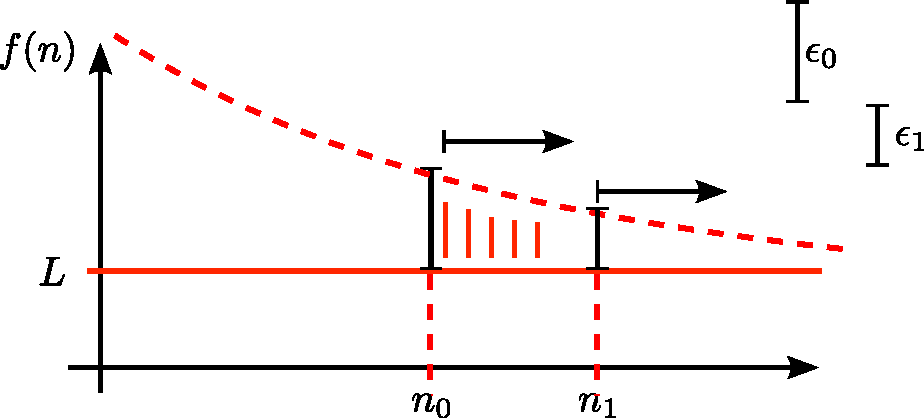
\includegraphics[width=0.9\textwidth]{Images/limits-epsilon.pdf}
    \end{center}
  \end{itemize}
\end{frame}

%%% ==========================================
%%% This should be at the END of the file !!!!!!
%%%
%%% Local Variables: 
%%% mode: latex 
%%% TeX-master: "~/TeX/TeXinput/Scripts/Algo-Data-EMS/Rolf-2016/AlgoDat/Lecture-3/Lecture.tex" 
%%% End: 
%%% ==========================================
